\documentclass{template}

% --- PACKAGES ---
% \usepackage[margin=1in, headheight=14pt, top=1.2in]{geometry}
% \usepackage{amsmath,amssymb}
% \usepackage{graphicx}
% \usepackage{enumitem}
% \usepackage{hyperref}
% \usepackage{fancyhdr}
% \usepackage{float}
\usepackage{xcolor}
\usepackage{mdframed}
\usepackage{etoolbox}
\usepackage{pdfpages}

\graphicspath{{attachments/}}

% --- TOGGLE FOR ANSWERS ---
% Set to \toggletrue{showanswers} to display answers.
% Set to \togglefalse{showanswers} to hide answers.
\newtoggle{showanswers}
\toggletrue{showanswers}

% --- CUSTOM SOLUTION ENVIRONMENT ---
\newmdenv[
  backgroundcolor=white,
  linecolor=blue!60!black,
  linewidth=1.5pt,
  topline=false,
  rightline=false,
  bottomline=false,
  leftmargin=2pt,
  innerleftmargin=10pt,
  innertopmargin=6pt,
  innerbottommargin=6pt,
  skipabove=8pt,
  skipbelow=8pt
]{solutionbox}

\newcommand{\solution}[1]{%
  \iftoggle{showanswers}{%
    \begin{solutionbox}
        #1
    \end{solutionbox}%
  }{}%
}

% \usepackage[]{opensans} % Loads Open Sans font family
% \newcommand{\solution}[1]{%
%   \iftoggle{showanswers}{%
%     \begin{solutionbox}
%         \fontsize{10}{12}\opensans #1
%     \end{solutionbox}%
%   }{}%
% }

\addbibresource{/Users/nathalieredick/repos/washu/notes/WashU.bib}


% --- HEADER & FOOTER CONFIGURATION ---
\pagestyle{fancy}
\fancyhf{}
\lhead{\textbf{EEPS 5534: Interior of the Earth}}
\rhead{\textbf{Problem Set 1}}
\cfoot{\thepage}


\title{\textbf{Problem Set 1}}
\author{Nathalie Redick}
\date{Due: Sept. 14, 2026}

\begin{document}

\maketitle
\thispagestyle{fancy}

\begin{enumerate}[label=\textbf{\arabic*.}]

    \item Three plates meet at a ridge-ridge-ridge triple junction as shown below. Each ridge is spreading symmetrically and orthogonally, and the full spreading rate between plates A and B is $5\text{ cm/yr}$. Calculate (either by graphing or trig):

    \begin{figure}[H]
        \centering
        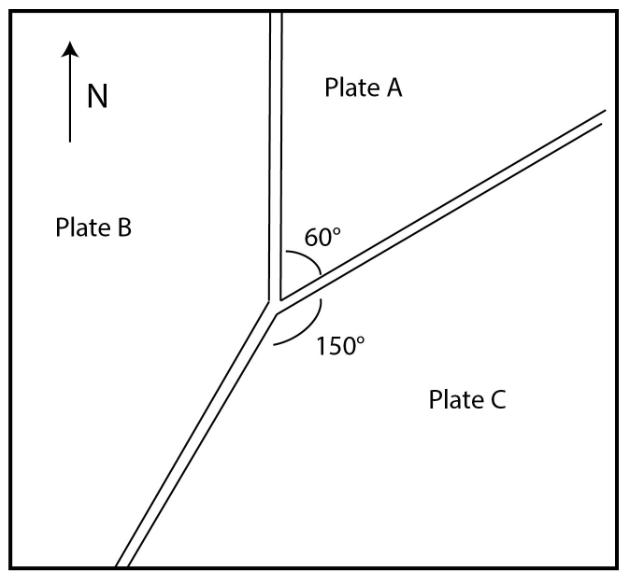
\includegraphics[width=0.45\textwidth]{hw1-q1.png}
    \end{figure}

    \begin{enumerate}[label=\Alph*)]
        \item The spreading rate of the other two ridges.
        \solution{
            The spreading rate of ridges $V_{AC}$ and $V_{BC}$ can be determined as follows:

            \begin{figure}[H]
                \centering
                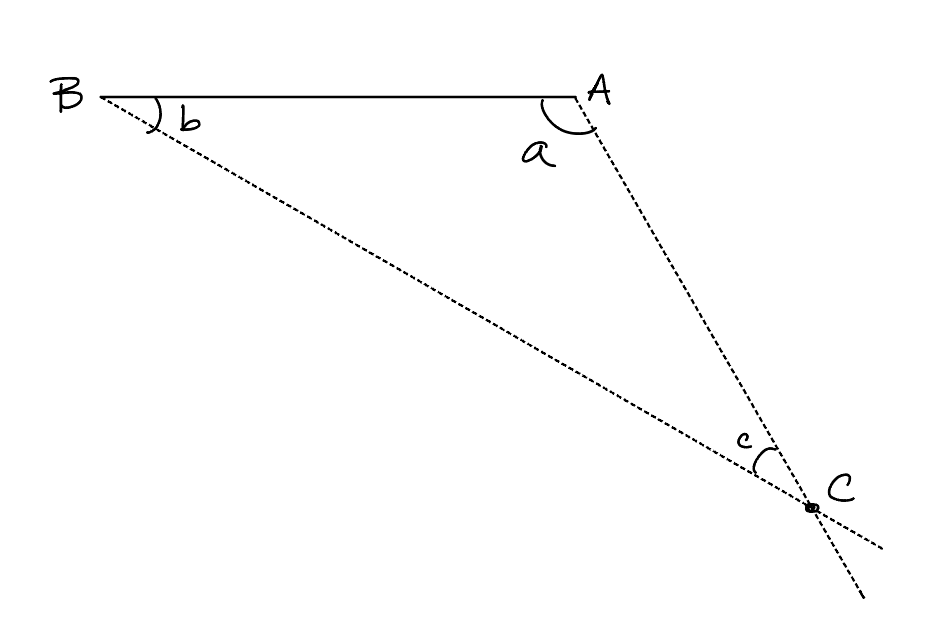
\includegraphics[width=0.5\textwidth]{hw1-q1a-ans.png}
                % \caption{Velocity triangle}
                \label{fig:q1a_1}
            \end{figure}

            % It is a required condition of all velocity triangles that $V_{BA} + V_{CB} + V_{AC} = 0$, where $V_{BA}$ is the velocity of plate B with respect to A, and so on (following the notation style of \textcite{turcotteGeodynamics2014}).\\

            Given the angles between spreading ridges $V_{AB}$-$V_{AC}$ and $V_{AC}$-$V_{BC}$, we can determine that $a=120\degree$ and $b,c=30\degree$.\\

            Using the law of sines, the spreading rates of the unknown ridges $V_{AC}$ and $V_{BC}$, where $V_{AC}$ is the velocity of plate A with respect to C, and so on (following the notation style of \textcite{turcotteGeodynamics2014}):

            \setlength{\jot}{10pt}
            \begin{align*}
                \frac{V_{AB}}{\sin c} &= \frac{V_{AC}}{\sin b} = \frac{V_{BC}}{\sin a} \\[4pt]
                \frac{5~\unit{cm/yr}}{\sin 30\degree} &= \frac{V_{AC}}{\sin 30\degree} = \frac{V_{BC}}{\sin 120\degree} \\[8pt]
                \frac{5~\unit{cm/yr}}{\sin 30\degree} &= \frac{V_{AC}}{\sin 30\degree}
                    & \frac{5~\unit{cm/yr}}{\sin 30\degree} &= \frac{V_{BC}}{\sin 120\degree} \\[8pt]
                V_{AC} &= \boxed{5~\unit{cm/yr}}
                    & V_{BC} &= \boxed{8.66~\unit{cm/yr}}
            \end{align*}
        }

        \item The velocity of the triple junction (direction and rate) relative to all three plates.
        \solution{
            The velocity of the triple junction relative to the plates can be determined graphically by drawing the perpendicular bisectors (since all three ridges are spreading centers) of each velocity line on the velocity triangle; the intersection (labelled TJ) is the location of the triple junction, and the lines between the triple junction and the plate points are the velocity lines of the triple junction relative to each respective plate.\\

            \begin{figure}[H]
                \centering
                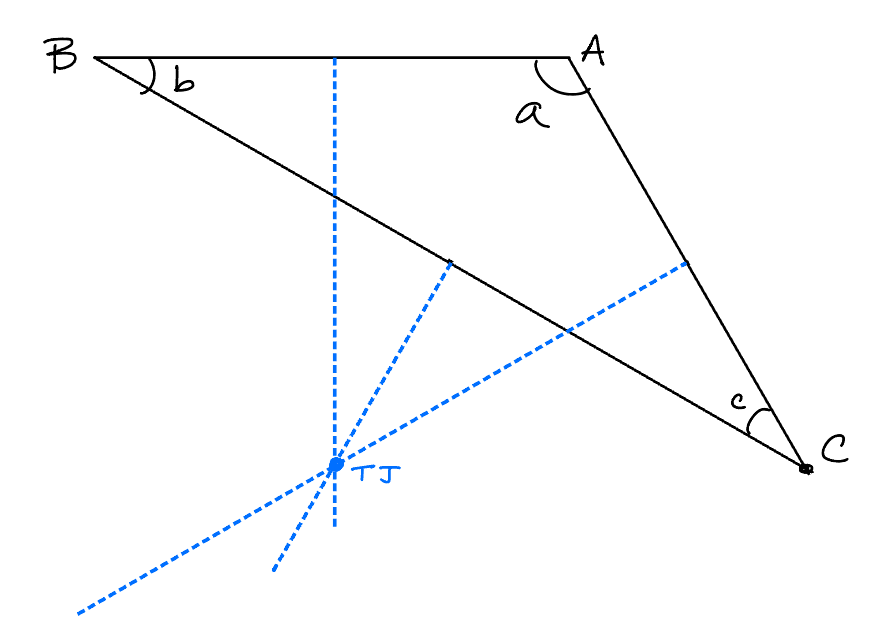
\includegraphics[width=0.5\textwidth]{hw1-q1b-ans}
                % \caption{CAPTION}
                \label{fig:hw1-q1b-ans}
            \end{figure}

            \begin{tabular}{lcc}
            \toprule
            Plate & Rate & Direction (azimuth from North) \\ \midrule
            A & $\sim5.1~\unit{cm/yr}$ & $210\degree$ \\ \addlinespace
            B & $\sim5.1~\unit{cm/yr}$ & $150\degree$ \\ \addlinespace
            C & $\sim5.1~\unit{cm/yr}$ & $270\degree$ \\ \bottomrule
            \end{tabular}\\

            The rate is measured from the length of the velocity line.
        }
    \end{enumerate}

    \item The San Andreas Fault system seems to have developed through something like the following scenario: Around 30 million years ago, the Farallon plate was subducting along the west coast of North America. Assume that the Pacific-Farallon spreading center was spreading in an E-W direction at $8\text{ cm/yr}$ and that the Farallon plate is moving at $8\text{ cm/yr}$ at a direction of N60$\degree$E relative to North America (The details of this problem have been simplified). Assume that the subduction zone trends at N15$\degree$W, and that spreading is orthogonal and symmetric.

    \begin{figure}[H]
        \centering
        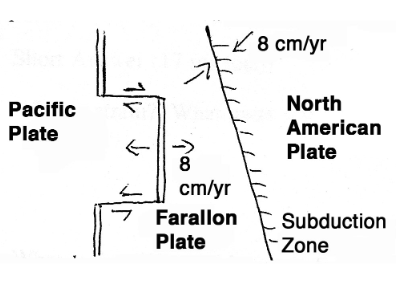
\includegraphics[width=0.45\textwidth]{hw1-q2b.png}
    \end{figure}

    \begin{enumerate}[label=\Alph*)]
        \item Diagram the plate velocities on a velocity vector diagram. What is the velocity of the Pacific Plate relative to North America? What is the velocity of the Pacific-Farallon spreading center relative to North America?

        \begin{figure}[H]
                \centering
                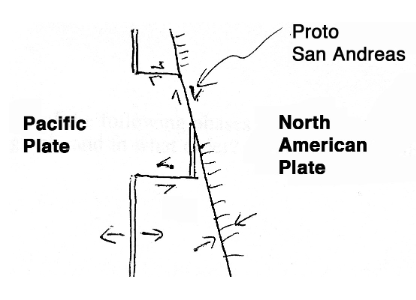
\includegraphics[width=0.45\textwidth]{hw1-q2a.png}
            \end{figure}

        \solution{
            \begin{figure}[H]
                \centering
                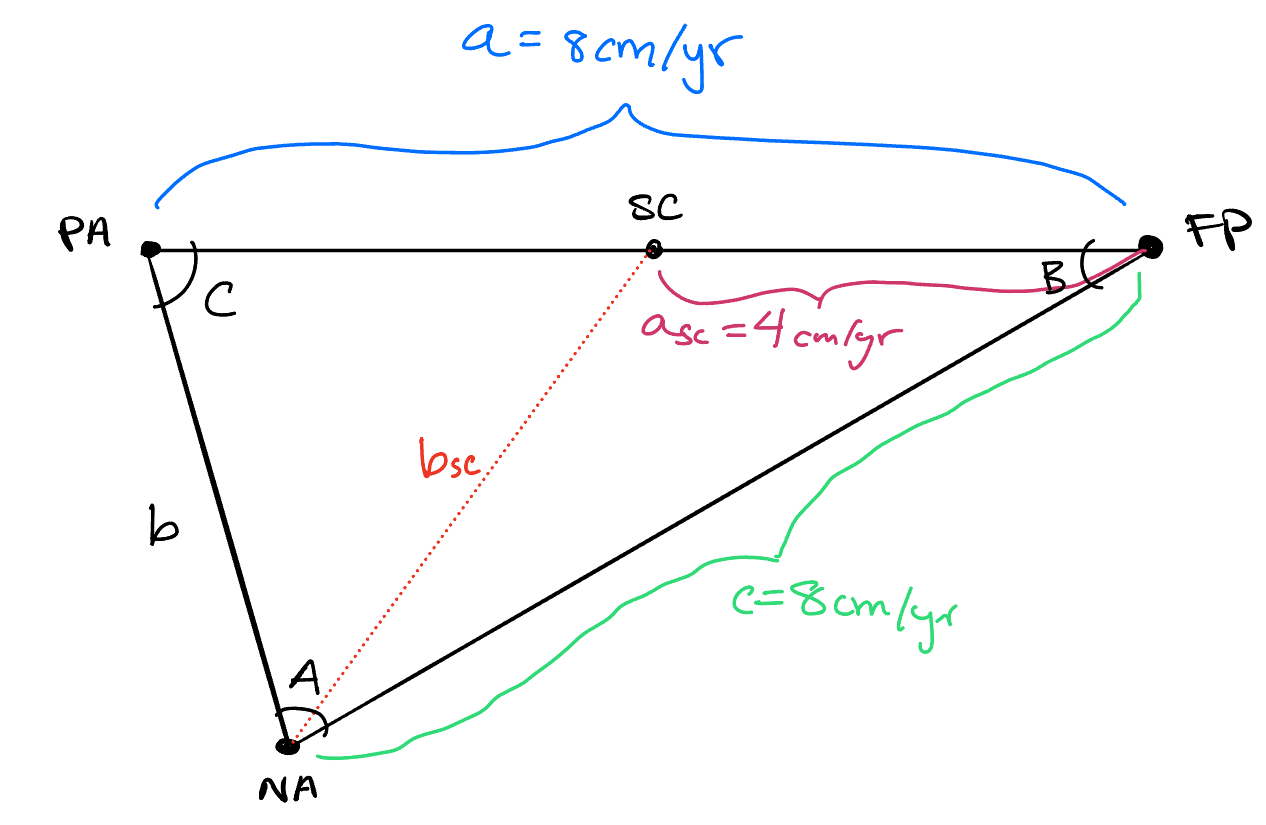
\includegraphics[width=0.7\textwidth]{hw1-q2a-ans}
                % \caption{CAPTION}
                \label{fig:hw1-q2a-ans}
            \end{figure}

            The relative plate velocities can be determined using the law of cosines.\\

            Velocity of the Pacific plate (PA) to the North American plate (NA):
            \begin{align*}
                % a^2 &= b^2 + c^2 - 2bc \cdot \cos A \\[6pt]
                b^2 &= a^2 + c^2 - 2ac \cos B \\
                b^2 &= 8^2 + 8^2 - 2(8)^2 \cos(30\degree) \\
                b &= \sqrt{17.15} \\
                b &= \boxed{\sim4.14 ~\unit{cm/yr}}
            \end{align*}

            Velocity of the Pacific-Farallon spreading center to the North American plate:
            \begin{align*}
                b_{\text{sc}}^2 &= a_{\text{sc}}^2 + c^2 - 2 a_{\text{sc}} c \cdot \cos(B) \\
                b_{\text{sc}}^2 &= 4^2 + 8^2 - 2(4 \cdot 8) \cos(30\degree) \\
                b_{\text{sc}} &= \sqrt{24.57} \\
                b_{\text{sc}} &= \boxed{\sim 4.96 ~\unit{cm/yr}}
            \end{align*}
        }

        \item Over a period of time the spreading center arrives at the subduction zone. A transform fault (the proto-San Andreas) forms where the ridge has hit the subduction zone. How many triple junctions are there in this system, and where are they located? Do a stability analysis for each of the triple junctions. Are the triple junctions stable and if so, what is the velocity of each of the triple junctions relative to North America? How fast is the San Andreas lengthening at this time?
        \solution{
            There are two triple junctions in the new configuration, located at the northern and southern ends of the proto-San Andreas fault.

            \begin{figure}[H]
                \centering
                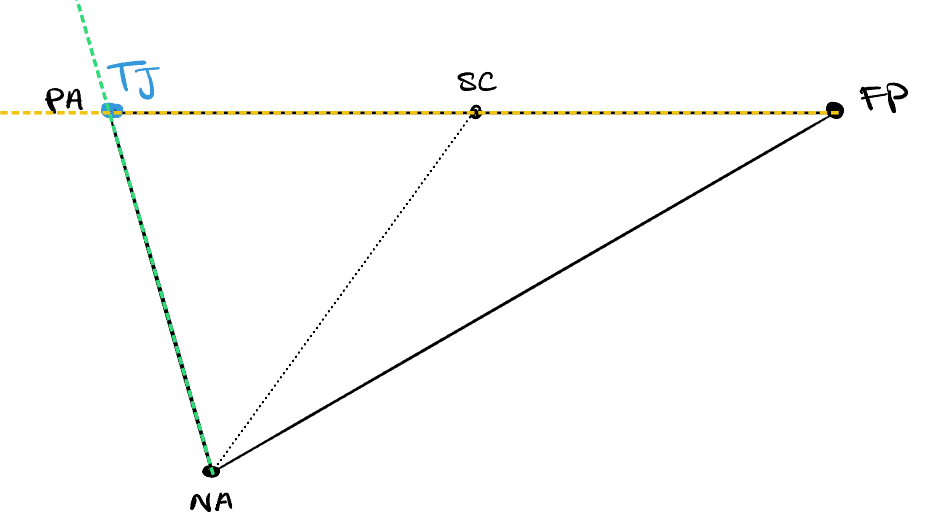
\includegraphics[width=0.6\textwidth]{hw1-q2b-ans1}
                \caption{TJ = northern triple junction, shown in blue. The location of the northern triple junction is determined by the intersection of the dashed lines; the green line for NA-FP is drawn parallel to the trench and intersecting the overriding plate (NA), and overlaps the NA-PA line. The yellow dashed line is for PA-FP.}
                \label{fig:hw1-q2b-ans1}
            \end{figure}

            Since all three dashed lines intersect, \textbf{the northern triple junction is stable}. The velocity of the southern triple junction relative to North America is $\sim 4.1 ~\unit{cm/yr}$ (measured from the velocity diagram).

            \begin{figure}[H]
                \centering
                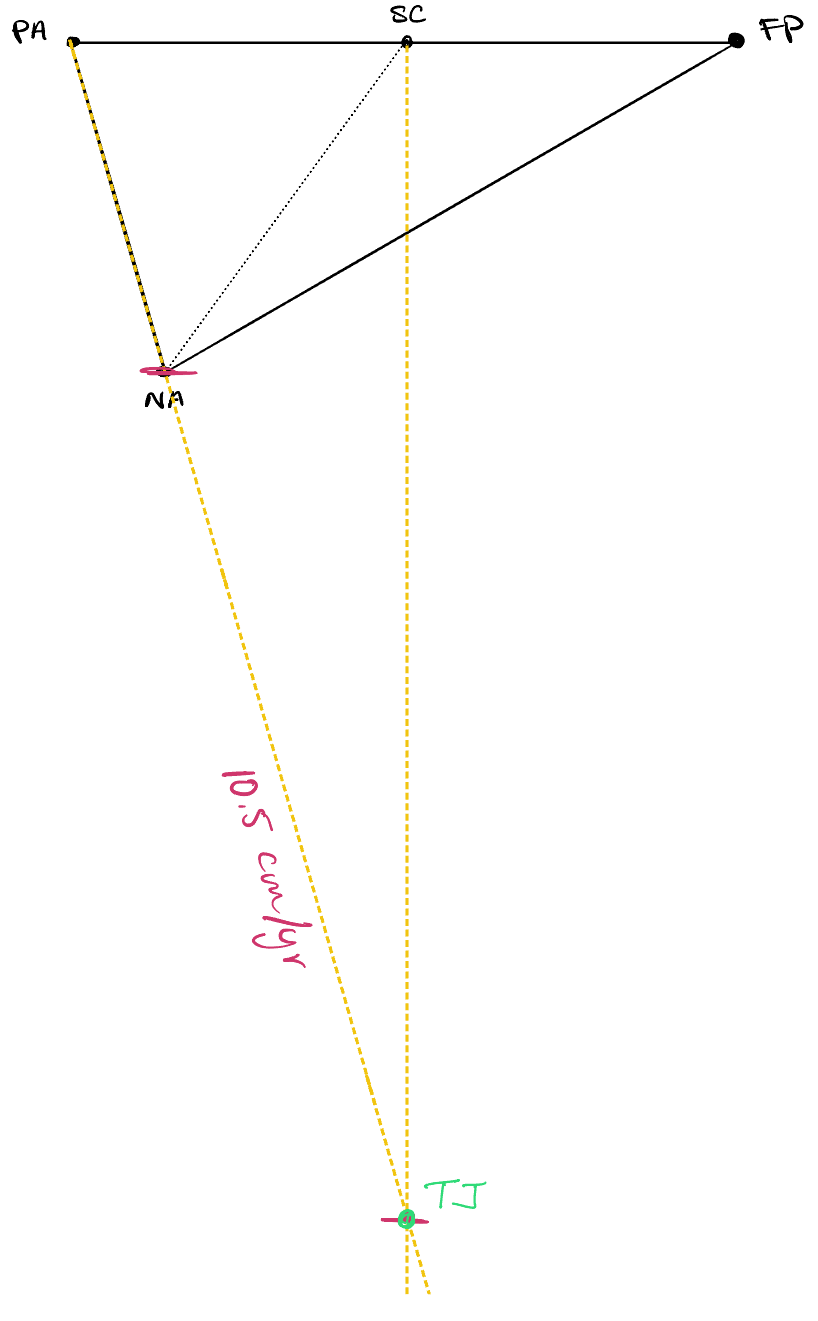
\includegraphics[width=0.6\textwidth]{hw1-q2b-ans2}
                \caption{TJ = southern triple junction, shown in green. The location of the southern triple junction is determined by the intersection of the dashed lines; the yellow dashed line for NA-FP is drawn parallel to the trench and intersecting the overriding plate (NA), and overlaps the NA-PA line. The other yellow dashed line is for PA-FP.}
                \label{fig:hw1-q2b-ans2}
            \end{figure}

            Since all three dashed lines intersect, \textbf{the southern triple junction is stable}. The velocity of the southern triple junction relative to North America is $\sim 10.5 ~\unit{cm/yr}$ (measured from the velocity diagram).\\

            At this point in time, the San Andreas lengthening at $4.1 ~\unit{cm/yr} + 10.5 ~\unit{cm/yr} =\boxed{\sim 14.6~\unit{cm/yr}}$
        }

        \item What will happen when the southern triple junction reaches the Farallon-Pacific transform fault? Do a stability analysis for the southern triple junction at this point. How fast will the San Andreas Fault be lengthening?

        \solution{
            \begin{figure}[H]
                \centering
                \begin{subfigure}[b]{0.48\textwidth}
                    \centering
                    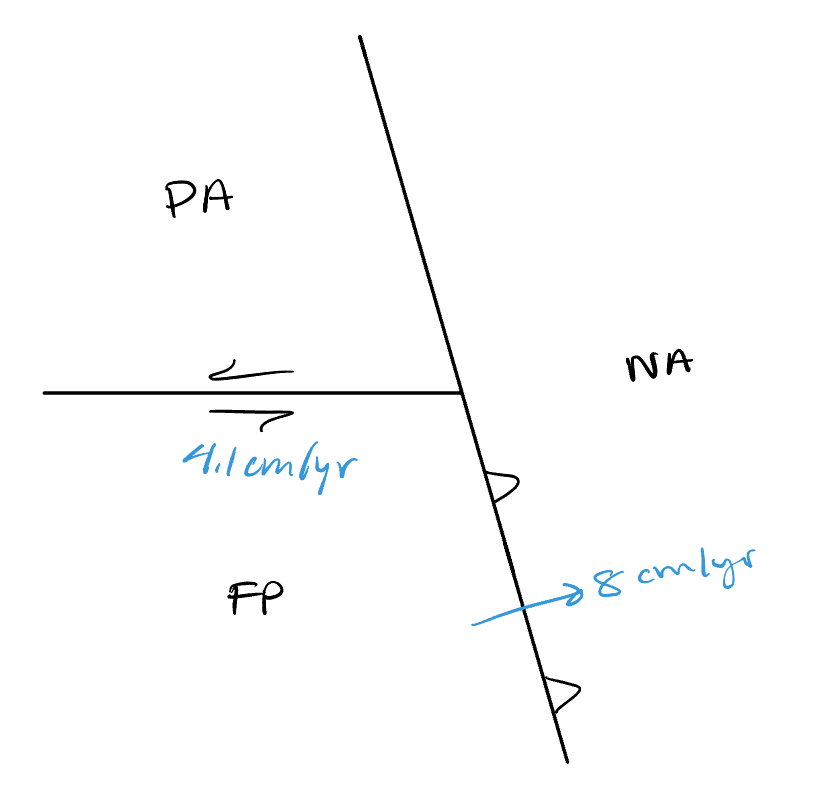
\includegraphics[width=\linewidth, height=2in, keepaspectratio]{hw1-q2c-ans1}
                    \caption{System configuration when the southern triple junction reaches the Farallon-Pacific transform fault.}
                    \label{fig:hw1-q2c-ans1}
                \end{subfigure}
                \hfill
                \begin{subfigure}[b]{0.48\textwidth}
                    \centering
                    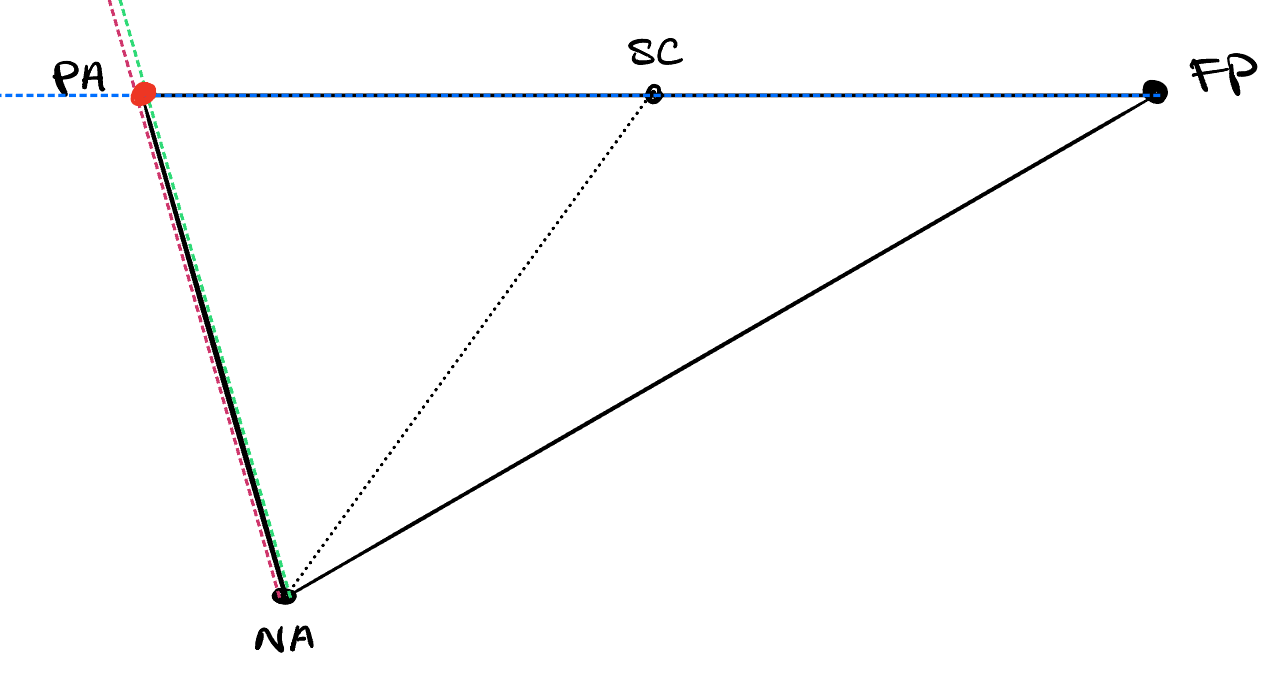
\includegraphics[width=\linewidth, height=2in, keepaspectratio]{hw1-q2c-ans2}
                    \caption{Stability analysis. All lines intersect on the red point at PA.}
                    \label{fig:hw1-q2c-ans2}
                \end{subfigure}
                % \caption{Combined figure caption}
                \label{fig:hw1-q2c-ans-combined}
            \end{figure}

            Since all the lines intersect in the stability analysis, the newly formed triple junction is stable.\\

            The new southern triple junction is now moving toward the northwest (towards PA) along the same trajectory as the northern triple junction at the same speed ($\sim 4.1~\unit{cm/yr}$), such that the \textbf{length San Andreas is not changing} over time at this point.
        }
    \end{enumerate}

    \item The planet Wegener, shown below, is comprised of the three plates A, B, and C with boundaries as shown (planet radius is $10{,}000\text{ km}$). The boundaries between A and B and between B and C are transform faults as shown. Both faults slip with a velocity of $10\text{ cm/yr}$.

    \begin{figure}[H]
        \centering
        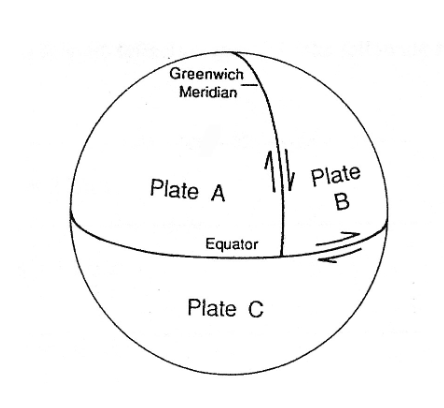
\includegraphics[width=0.45\textwidth]{hw1-q3.png}
    \end{figure}

    \begin{enumerate}[label=\Alph*)]
        \item Is the triple junction on the near side of the planet stable? If not, what will it probably look like in a few million years? What about the triple junction on the far side of the planet?

        \solution{
            The triple junction on the near side of the planet is \textbf{not stable}, because you cannot construct a velocity triangle for this triple junction:

            \begin{figure}[H]
                \centering
                \begin{minipage}[t]{0.46\textwidth}
                    \centering
                    % \textbf{Initial Unstable Junction} \\[4pt]
                    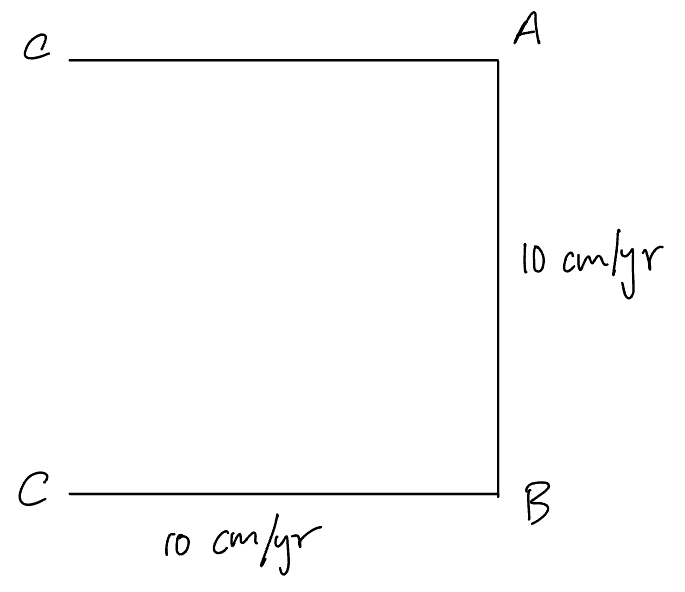
\includegraphics[width=\linewidth, height=2.2in, keepaspectratio]{hw1-q3a-ans1}
                    \caption{Unclosed velocity diagram based on the near side triple junction.}
                    \label{fig:hw1-q3a-ans1}
                \end{minipage}%
                \hfill
                \begin{minipage}[t]{0.46\textwidth}
                    \centering
                    % \textbf{Evolved Junction Geometry} \\[4pt]
                    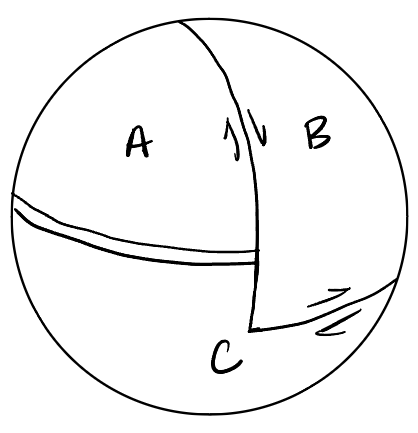
\includegraphics[width=\linewidth, height=2.2in, keepaspectratio]{hw1-q3a-ans2}
                    \caption{In a few million years, the near side triple junction may look like this. Deduced spreading center between A-C shown.}
                    \label{fig:hw1-q3a-ans2}
                \end{minipage}
            \end{figure}

            The triple junction on the far side of the planet is stable:

            \begin{figure}[H]
                \centering
                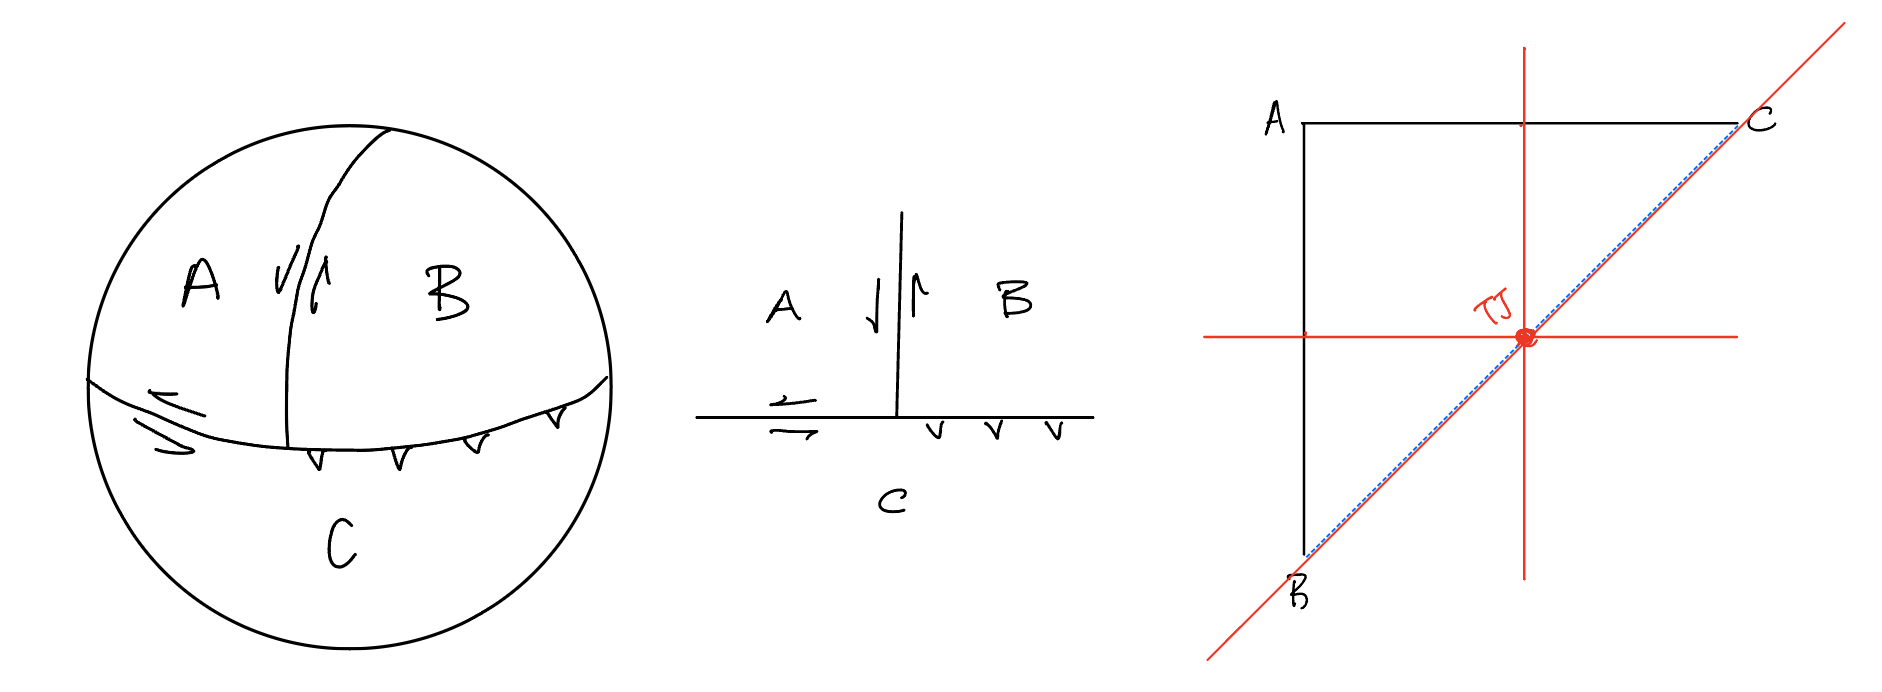
\includegraphics[width=\textwidth]{hw1-q3a-ans3}
                \caption{Convergent boundary between B-C on the far side of the planet determined in order to balance the plate motions.}
                \label{fig:hw1-q3a-ans3}
            \end{figure}
        }
        \newpage
        \item Find the geographic location of the Euler vector describing motion between plates A and C (give the geographic coordinates of the pole and the rotation rate).

        \solution{
            The Euler vectors for transform boundaries lie perpendicular to the motion along small circles centered at the poles of rotation \parencite{turcotteGeodynamics2014}, such that:

            \begin{itemize}
                \item The transform boundary $AB$ (which lies along the Greenwich Meridian) has an Euler vector $\vec{\omega}_{AB}$ centered at $(0\degree\text{ N}, 0\degree\text{ E/W})$ along the equator.
                \item The other transform boundary $BC$ (along the Equator) has an Euler vector $\vec{\omega}_{BC}$ centered at the geographic North Pole $(90\degree\text{ N}, 0\degree\text{ E})$.
            \end{itemize}

            Since both boundaries lie at an angular distance of $\theta = 90\degree$ from their respective poles ($\sin 90\degree = 1$), the magnitude of angular velocity is:
            \setlength{\jot}{8pt}
            \begin{align*}
                v_{AB} = v_{BC} &= \omega R \sin\theta = 10 ~\unit{cm/yr} \\[4pt]
                \omega_{AB} = \omega_{BC} &= \frac{v}{R} = \frac{10 ~\unit{cm/yr}}{\num{1e9} ~\unit{cm}} = \num{1e-8} ~\unit{rad/yr}
            \end{align*}

            % In a Cartesian coordinate system where $\hat{i}$ points to $(0\degree\text{ N}, 0\degree\text{ E})$ and $\hat{k}$ points to $(90\degree\text{ N})$, the vector closure condition yields:
            % \begin{align*}
            %     \vec{\omega}_{AC} &= \vec{\omega}_{AB} + \vec{\omega}_{BC} \\[4pt]
            %     \vec{\omega}_{AC} &= \left( \num{1e-8}\hat{i} + 0\hat{j} + \num{1e-8}\hat{k} \right) ~\unit{rad/yr}
            % \end{align*}

            Then, the position and magnitude of the Euler pole for $AC$ can be calculated as:
            \begin{align*}
                \lambda_{AC} &= \arctan\left(\frac{\omega_{BC}}{\omega_{AB}}\right) = \arctan\left(\frac{\num{1e-8}}{\num{1e-8}}\right) = \arctan(1) = \boxed{45\degree\text{ N}} \\[4pt]
                \phi_{AC} &= \arctan2(0, \omega_{AB}) = \arctan2(0, \num{1e-8}) = \boxed{0\degree\text{ E}} \\[4pt]
                \|\vec{\omega}_{AC}\| &= \sqrt{\omega_{AB}^2 + \omega_{BC}^2} = \sqrt{(\num{1e-8})^2 + (\num{1e-8})^2} = \sqrt{2} \times \num{1e-8}\\ &\approx \boxed{1.414 \times 10^{-8}~\unit{rad/yr}\quad\text{\bf OR}\quad 1.414 \times 10^{-8}\cdot \frac{180}{\pi} \approx 8.1\times 10^{-7}~\unit{\degree/yr}}
            \end{align*}
        }

        \item Describe the tectonic nature of the boundary between A and C, including the part of the boundary on the far side of the planet. If the planet has magnetic field reversals, where would sea-floor spreading magnetic anomalies be found? Where would the maximum spreading rate be found?
        \solution{
            On the near side of the planet, the boundary between A and C is a spreading center (shown in Fig~\ref{fig:hw1-q3a-ans2}). Therefore, sea-floor spreading magnetic anomalies would be found on either side of ridge AC. The maximum spreading rate would be along ridge AC closet to the near side triple junction where the spread distance along the AB transform from the near to far side triple junctions is longest.
        }
    \end{enumerate}

    \item The hotspot reference frame (such as model HS3-NUVEL1A; Gripp and Gordon 2002) represents plate motions relative to hotspots assuming that hotspots are fixed relative to each other. The no-net rotation reference frame (such as NNR-MORVEL56; Argus et al., 2011) also attempts to represent plate motions relative to the mantle. You can compute the plate velocities at any point using the NGF plate motion calculator (\url{https://www.unavco.org/software/geodetic-utilities/plate-motion-calculator/plate-motion-calculator.html}). You just enter the lat, lon of the location where you want the velocity calculated, put in the name of the model, and make sure the reference is correct (HS for hotspot, NNR for no-net rotation).

    Now use this tool to investigate whether the following possible hotspots indeed track with the expected velocities. In each case, calculate and write down the velocity with the two models above, and then plot the expected locations of past volcanism from the two models over the past $\sim 10\text{ Ma}$. Then comment on whether the volcanism is consistent with the HS or NNR plate motion models (or both).

    \begin{enumerate}[label=\Alph*)]
        \item Yellowstone. You will want to use a map showing past caldera locations such as \url{https://www.isu.edu/digitalgeologyidaho/yellowstone-srp/}.
        \solution{
            \begin{figure}[H]
                \centering
                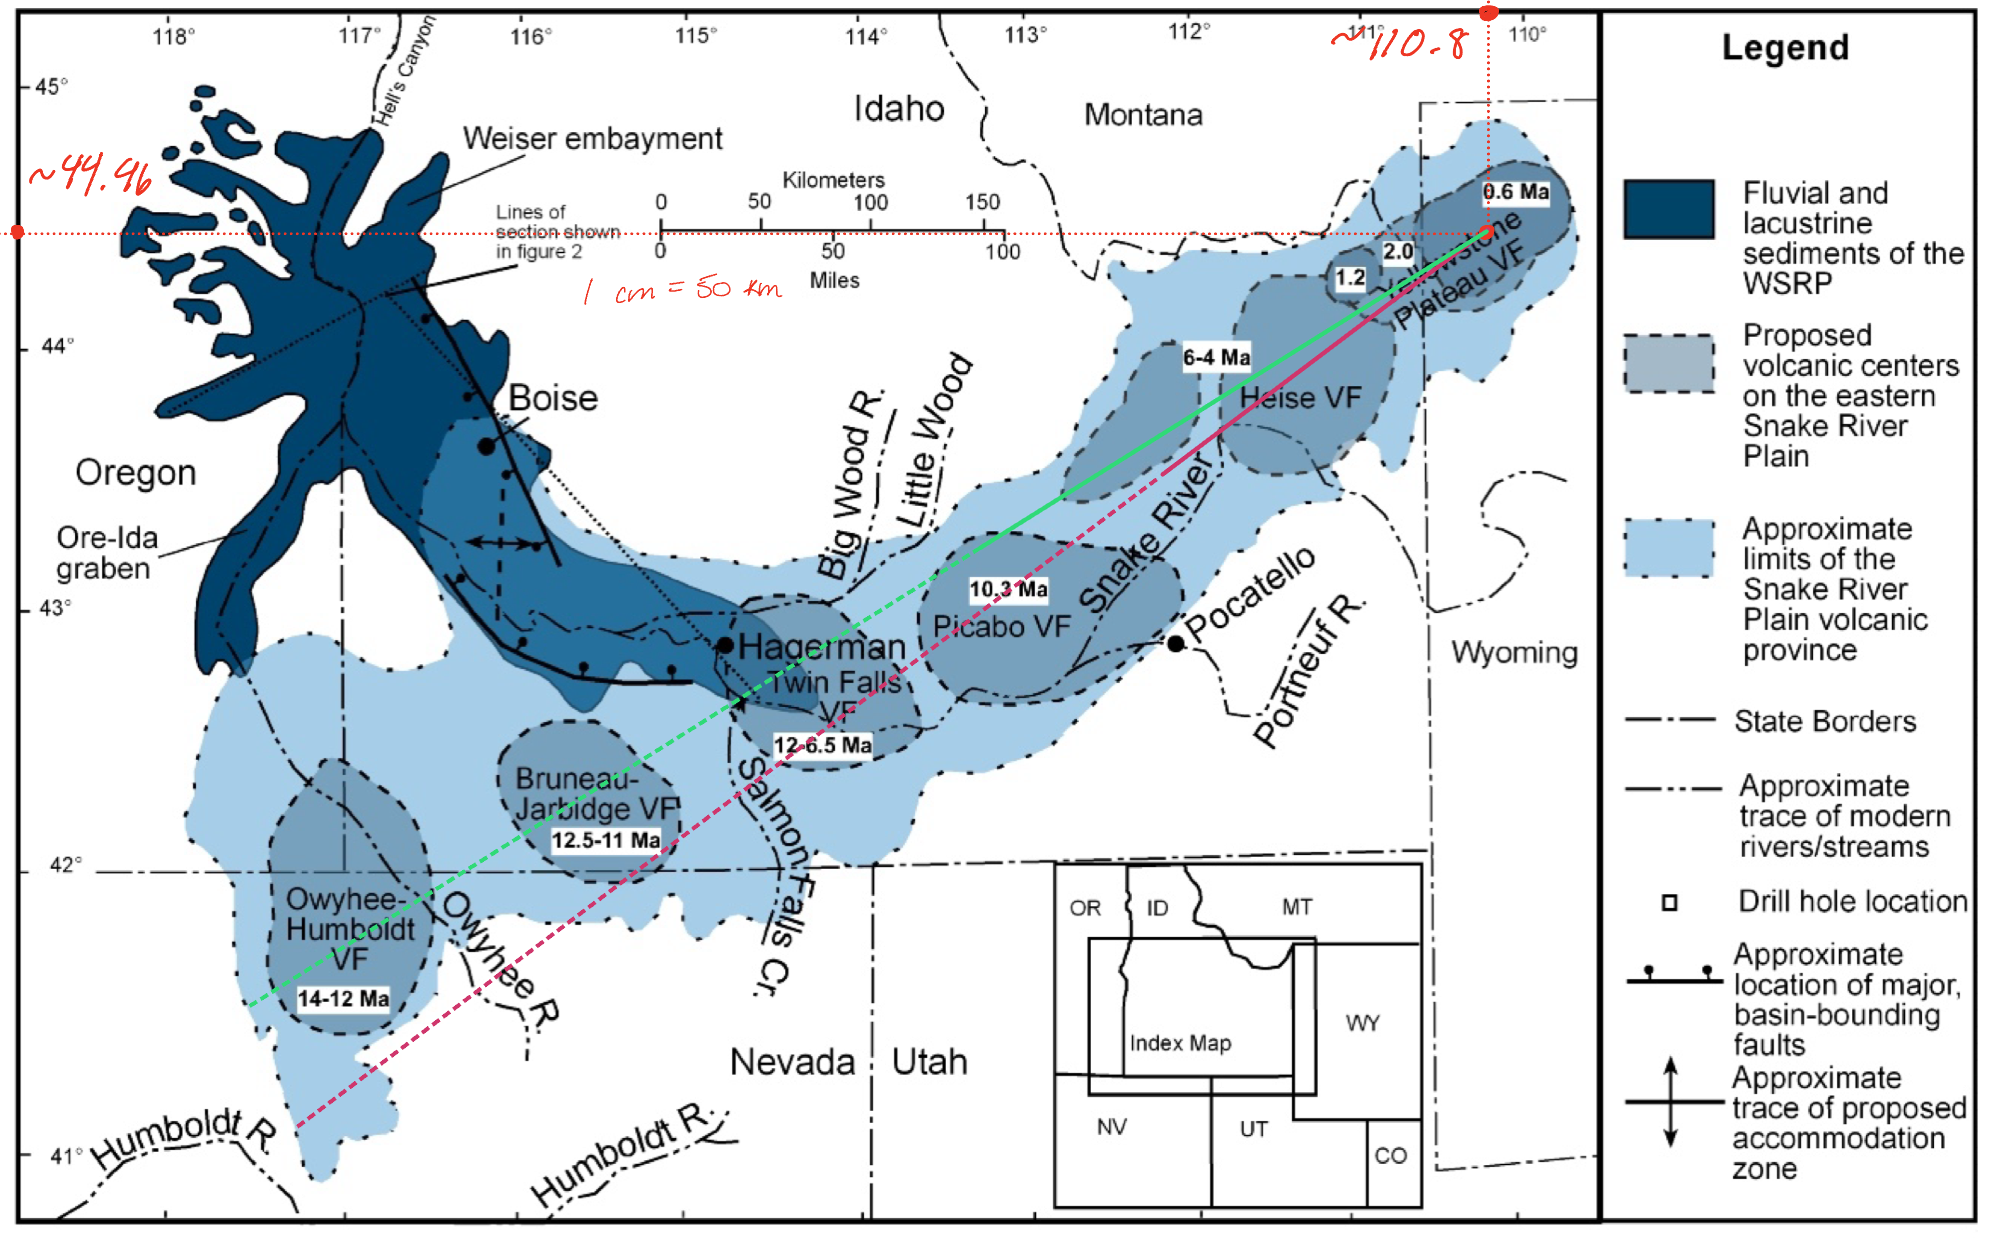
\includegraphics[width=0.9\textwidth]{hw1-q4a-map}
                \caption{Solid line shows the 10 Ma projection; dashed line projects beyond. The green line is the HS3-NUVEL1A estimate, and the pink line is the NNR-MORVEL56 estimate.}
                \label{fig:hw1-q4a-map}
            \end{figure}

            I used the map to estimate the location of the near-modern 0.6 Ma hotspot center at (110.8, 44.46), which results in estimates of:

            \begin{table}[H]
                \centering
                % \caption{Plate motion velocity vectors for Yellowstone hotspot models.}
                \small
                \begin{tabular}{ccrrlll}
                    \toprule
                    \textbf{Lon ($^\circ$E)} & \textbf{Lat ($^\circ$N)} & \textbf{Speed (mm/yr)} & \textbf{Az} (°cw N) & \textbf{Plate (Ref)} & \textbf{Model} \\
                    \midrule
                    -110.80 & 44.46 & 18.05 & 237.59 & NA(NNR) & NNR-MORVEL56 \\
                    -110.80 & 44.46 & 26.70 & 232.90 & NA(HS) & HS3-NUVEL1A  \\
                    \bottomrule
                \end{tabular}
            \end{table}

            The map was sized at 1 cm = 50 km; the lengths of the lines (for 10 Ma) are as follows:
            \begin{align*}
                % Left Column: HS3-NUVEL1A
                \frac{18.05\,\unit{mm}}{1\unit{E}6\,\unit{mm/km}} &= 180.5\,\unit{km}
                &
                % Right Column: NNR-MORVEL56
                \frac{26.70\,\unit{mm}}{1\unit{E}6\,\unit{mm/km}} &= 267.0\,\unit{km} \\[1.5em]
                %
                \frac{1\,\unit{cm}}{50\,\unit{km}} &= \frac{x\,\unit{cm}}{180.5\,\unit{km}}
                &
                \frac{1\,\unit{cm}}{50\,\unit{km}} &= \frac{x\,\unit{cm}}{267.0\,\unit{km}} \\[1.5em]
                %
                \frac{180.5}{50} &= 3.61\,\unit{cm}
                &
                \frac{267.0}{50} &= 5.34\,\unit{cm}
            \end{align*}

            The hotspot reference frame estimate provides a better fit to both the trajectory and displacement of the track over time. The NNR estimate severely underestimates the distance, but does a decent job with the trajectory. The HS reference frame is a good match to the magnitude of displacement, and is more in line with the long-range trajectory of the hotspot track when the line is projected beyond 10 Ma (shown as a dashed line).
        }

        \item Hawaii. (there are several maps with volcanism ages in the Wikipedia article ``List of volcanoes in the Hawaiian-Emperor seamount chain'')
        \solution{
            Using Kilauea on the Big Island as the reference point since it is

            \begin{figure}[H]
                \centering
                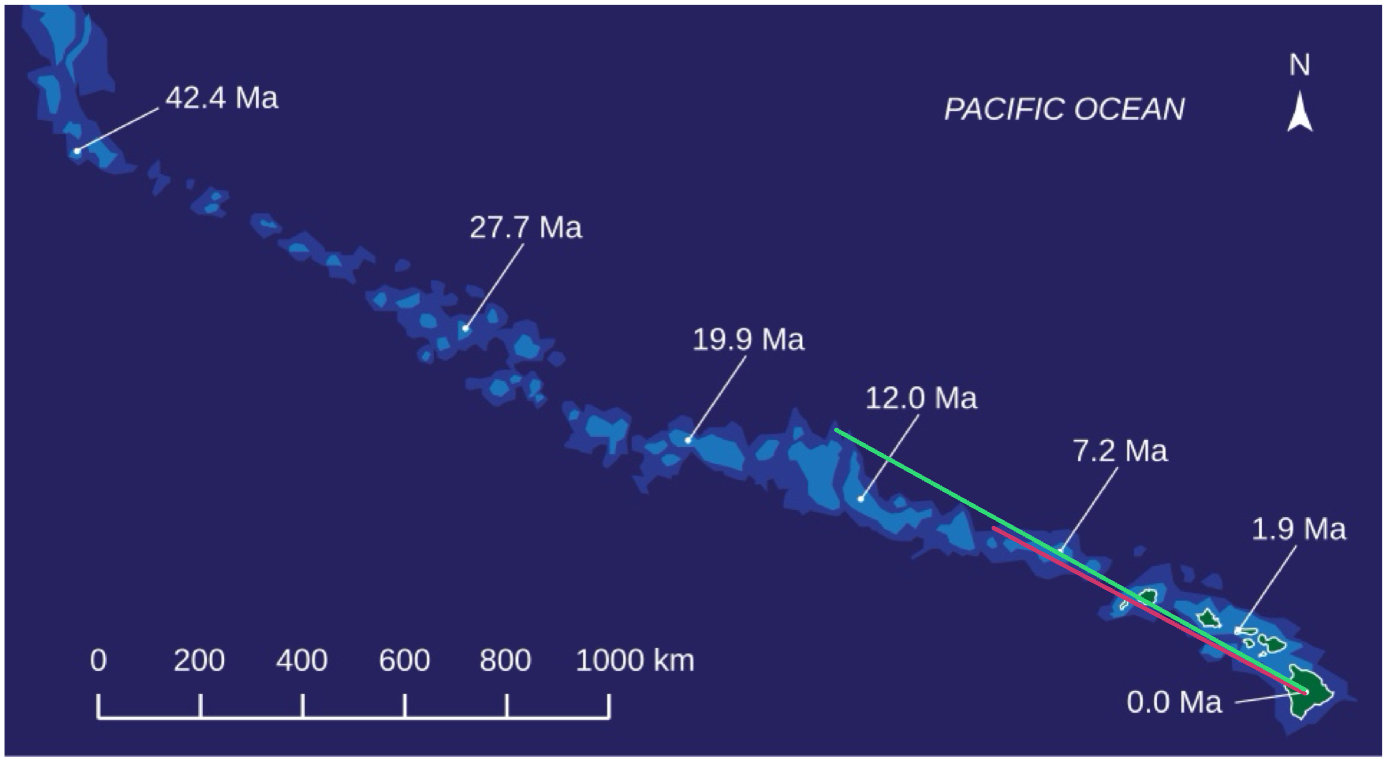
\includegraphics[width=\textwidth]{hw1-q4b-map}
                \caption{The green line is the HS3-NUVEL1A estimate, and the pink line is the NNR-MORVEL56 estimate.}
                \label{fig:hw1-q4b-map}
            \end{figure}

            % Lon(°E)      Lat(°N)      Evel(mm/yr) Nvel(mm/yr)  Plate(Reference) Model Site
            % -155.280000  19.420000     -58.63      32.07  PA(NNR) HS3-NUVEL1A
            % -155.280000  19.420000     -61.23      32.23  PA(NNR) NNR-MORVEL56

            \begin{table}[H]
                \centering
                % \caption{Plate motion velocity vectors for Yellowstone hotspot models.}
                \small
                \begin{tabular}{ccrrlll}
                    \toprule
                    \textbf{Lon ($^\circ$E)} & \textbf{Lat ($^\circ$N)} & \textbf{Speed (mm/yr)} & \textbf{Az} (°cw N) & \textbf{Plate (Ref)} & \textbf{Model} \\
                    \midrule
                    -155.28 & 19.42 & 69.19 & 297.77 & PA(NNR) & NNR-MORVEL56 \\
                    -155.28 & 19.42 & 103.81 & 298.68 & PA(HS) & HS3-NUVEL1A  \\
                    \bottomrule
                \end{tabular}
            \end{table}

            The map was sized at 1 cm = 200 km; the lengths of the lines (for 10 Ma) are as follows:
            \begin{align*}
                % Left Column: HS3-NUVEL1A
                \frac{69.19\,\unit{mm}}{1\unit{E}6\,\unit{mm/km}} &= 691.9\,\unit{km}
                &
                % Right Column: NNR-MORVEL56
                \frac{103.81\,\unit{mm}}{1\unit{E}6\,\unit{mm/km}} &= 1038.1\,\unit{km} \\[1.5em]
                %
                \frac{1\,\unit{cm}}{200\,\unit{km}} &= \frac{x\,\unit{cm}}{691.9\,\unit{km}}
                &
                \frac{1\,\unit{cm}}{200\,\unit{km}} &= \frac{x\,\unit{cm}}{1038.1\,\unit{km}} \\[1.5em]
                %
                \frac{691.9}{200} &= 3.46\,\unit{cm}
                &
                \frac{1038.1}{200} &= 5.19\,\unit{cm}
            \end{align*}

            % Solid line shows the 10 Ma projection; dashed line projects beyond. The green line is the HS3-NUVEL1A estimate, and the pink line is the NNR-MORVEL56 estimate.

            The NNR estimate (pink) shows a much better fit to the expected amount of spatial displacement over time relative to the HS3 estimate; however, both lines have a comparable fit to the expected trajectory of the plate motion (projecting slightly too far north).
        }

        \item Samoa (see Hart et al., Earth \& Planetary Science Letters, 2004, figure 1A). Current location of the hotspot is thought to be Vailulu'u seamount.
        \solution{
            \begin{figure}[H]
                \centering
                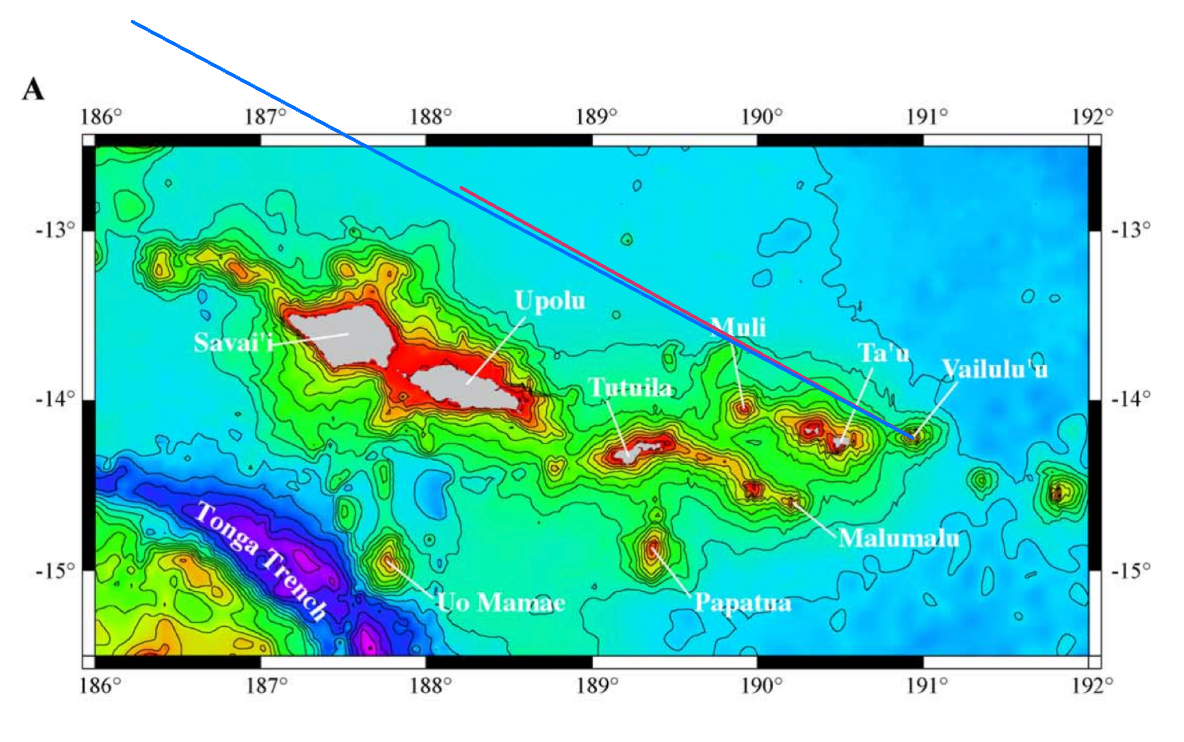
\includegraphics[width=0.8\textwidth]{hw1-q4c-map}
                \caption{The blue line is the HS3-NUVEL1A estimate, and the pink line is the NNR-MORVEL56 estimate.}
                \label{fig:hw1-q4c-map}
            \end{figure}

            \begin{table}[H]
                \centering
                % \caption{Plate motion velocity vectors for Yellowstone hotspot models.}
                \small
                \begin{tabular}{ccrrlll}
                    \toprule
                    \textbf{Lon ($^\circ$E)} & \textbf{Lat ($^\circ$N)} & \textbf{Speed (mm/yr)} & \textbf{Az} (°cw N) & \textbf{Plate (Ref)} & \textbf{Model} \\ % 151
                    \midrule
                    -14.2150 & -169.0583 & 68.62 & 297.15 & PA(NNR) & NNR-MORVEL56 \\
                    -14.2150 & -169.0583 & 117.13 & 298.26 & PA(HS) & HS3-NUVEL1A  \\ % 152
                    \bottomrule
                \end{tabular}
            \end{table}

        The map was sized at 2 cm = 111 km (using the estimate that $1\degree \approx 111~\unit{km}$); the lengths of the lines (for 5 Ma, in order to fit on the map) are as follows:
            \begin{align*}
                % Left Column: NNR-MORVEL56
                \frac{68.62\,\unit{mm}}{1\unit{E}6\,\unit{mm/km}} \times 0.5 &= 343.1\,\unit{km}
                &
                % Right Column: HS3-NUVEL1A
                \frac{117.13\,\unit{mm}}{1\unit{E}6\,\unit{mm/km}} \times 0.5 &= 585.65\,\unit{km} \\[1.5em]
                %
                \frac{2\,\unit{cm}}{111\,\unit{km}} &= \frac{x\,\unit{cm}}{343.1\,\unit{km}}
                &
                \frac{2\,\unit{cm}}{111\,\unit{km}} &= \frac{x\,\unit{cm}}{585.65\,\unit{km}} \\[1.5em]
                %
                \frac{343.1 \times 2}{111} &= 6.18\,\unit{cm}
                &
                \frac{585.65 \times 2}{111} &= 10.55\,\unit{cm}
            \end{align*}

            The volcanism is relatively more consistent with the NNR model; however, neither are very accurate at this location.
        }
    \end{enumerate}

    \item Modeling bulk Earth compositions with chondrites:

    As we have seen in class, modeling the Earth's bulk composition with chondrites is a multi-variable process, and to be done with any chance of success must take into account elemental and isotopic abundances as well as potential assumptions about stochastic events in Earth history, and an understanding of early solar system dynamics. That being said, there is a lot of value to trying to build simple models to bolster ones understanding.

    \begin{enumerate}[label=\Alph*)]
        \item For this problem, estimate a composition of BSE using compositions of CI and EL type chondrites. CI chondrites overall match the composition of the Sun (solar system), and EL chondrites represent one of the best isotopic matches for bulk Earth. For this exercise, please use constraints on the core size to determine the amount of Fe and Ni that would partition into the BSE. Do a \textit{best fit} calculation assuming the core of the earth is 30\% the mass of the earth, and that BSE is 70\%. You can assume, for the sake of this calculation, that all sulfur goes into the core as elemental sulfur (a way oversimplified assumption, but will do for this exercise).
        % \solution{
        %     % todo ADD YOUR ANSWER HERE
        %     Write your answer for 5A here...
        % }

        \item Compare the compositions for BSE calculated in part 1 to the BSE estimate of McDonough and Sun (1995), based on physical samples, which is provided. Do the CI or EL chondrites capture the correct composition? If not, what elements or element ratios seem to be the most problematic. What are some reasons for the mismatch?
        % \solution{
        %     % todo ADD YOUR ANSWER HERE
        %     Write your answer for 5B here...
        % }

        \item What assumptions did you have to make in order to do this calculation, and how could the results differ if you changed or relaxed some of these assumptions? For example, we have done these calculations in order to match the \textit{current} core size of Earth, however EL chondrites are very reduced and have little \ce{FeO} in the silicate fraction. If the Earth was built of EL components, what would this tell you about the oxidation history of the planet? What geologic events/processes could also exert control on BSE composition, not just meteorite bulk composition?
        % \solution{
        %     % todo ADD YOUR ANSWER HERE
        %     Write your answer for 5C here...
        % }
    \end{enumerate}

    \solution{
        Answers for 5A--C where computed in a Jupyter notebook, which is attached as at the end as a PDF.
    }

    \vspace{0.5em}

    \begin{table}[H]
        \centering
        \begin{tabular}{l S[table-format=2.2] S[table-format=2.2] l S[table-format=2.3]}
            \toprule
            & {\parbox{3.5cm}{\centering Jajh deh Kot Lalu \\ \small (Mason 1966) \\ EL6 (S estimated) \\ wt\%}}
            & {\parbox{3.0cm}{\centering Palme and \\ Jones (2005) \\[1.2ex] CI wt\%}}
            &
            & {\parbox{3.0cm}{\centering McDonough and \\ Sun (1995) \\[1.2ex] wt\%}} \\
            \midrule
            Na & 1.08 & 1.14 & \ce{Na2O}  & 0.36 \\
            Mg & 22.3 & 21.9 & \ce{MgO}   & 37.8 \\
            Al & 1.68 & 1.94 & \ce{Al2O3} & 4.45 \\
            Si & 32.6 & 24.4 & \ce{SiO2}  & 45 \\
            S  & 3.10 & 3.19 & \ce{K2O}   & 0.029 \\
            K  & 0.08 & 0.12 & \ce{CaO}   & 3.55 \\
            Ca & 1.52 & 2.13 & \ce{TiO2}  & 0.2 \\
            Ti & 0.08 & 0.10 & \ce{Cr2O3} & 0.384 \\
            Cr & 0.35 & 0.60 & \ce{FeO}   & 8.05 \\
            Fe & 35.2 & 42.0 & \ce{NiO}   & 0.25 \\
            Ni & 2.05 & 2.46 &            & \\
            \bottomrule
        \end{tabular}
    \end{table}

\end{enumerate}

\section*{Acknowledgments}
Some LaTeX typesetting/formatting, conversion of table for question 5 to CSV format, and code clean-up assistance provided by Google Gemini (September 2026 version).

\singlespacing
\printbibliography[title={References}]

\includepdf[pages=-]{"hw1-q5.pdf"}

% \newpage

\end{document}